%%% Preamble
\documentclass[paper=a4, fontsize=11pt]{article}



% font
\usepackage{palatino}
%\documentclass{article}
\usepackage[utf8]{inputenc}
\usepackage{siunitx}
\usepackage{listings}
\usepackage{gensymb}
%\usepackage{tabu}
%\usepackage{tabulary}
%\usepackage{array}
%\usepackage{geometry}
\usepackage{pdflscape}
\usepackage{float}
\usepackage[backend=biber,style=nature,%sorting=ynt
]{biblatex}
%\addbibresource{barley1.bib}
\addbibresource{barley.bib}


%%% graph
\usepackage{graphicx}
\graphicspath{ {./images/}}
\usepackage{wrapfig}
\usepackage{lscape}


%%% KU template
%\usepackage[english, ku, large]{ku-frontpage}
%\assignment{}
%\subtitle{Project outside Course Scope, MSc}



\usepackage[acronym]{glossaries}
\makeglossaries


\title{Discovering Barley Intake Biomarkers in Urine by UPLC-MS Based Untargeted Metabolomics}
\author{Tu Hu \thanks{supervisor: Gözde Gürdeniz}}
\date{November 2018}

\begin{document}

\maketitle
\begin{abstract}
    Barley is one of the most produced cereal grains. Food industry and customers recently showed increasing interest to use barley as healthy food ingredients. 
However, its health beneficial effects has not been clarified yet due to lack of subjective measurement of food exposure. 
An UPLC-MS based untargeted metabolomics study was performed to discover biomarkers of barley intake in urine from a randomized cross-over study in 14 healthy volunteers having consumed whole grain barley bread and whole grain wheat bread.
6 candidate markers were proposed and putatively identified: 
two of them were reported with molecular weight and possible formulas. Other two were putatively identified as glucoronate conjugates. One was putatively identified as polyphenol or phenol metabolite. The rest one was identified as phytosterol metabolite.
Taken together, promising candidate biomarkers of barley intake appear to be phytochemicals and their metabolites. 
For cereal products, unique phytochemical metabolome pattern could indicate their intakes.

\end{abstract}

\clearpage
\tableofcontents

\newacronym{cvd}{CVD}{cardiovascular diseases}
\newacronym{tc}{TC}{Total Cholesterol}
\newacronym{ldlc}{LDL-C}{Low Density Lipoprotein Cholesterol}
\newacronym{hdlc}{HDL-C}{High Density Lipoprotein Cholesterol}
\newacronym{tg}{TG}{Triglycerides}
\newacronym{crp}{CRP}{C-Reactive Protein}
\newacronym{wbb}{WBB}{Whole Barley Bread}
\newacronym{wwb}{WWB}{Whole Wheat Bread}
\newacronym{bfis}{BFIs}{Biomarkers of Food Intake}
\newacronym{lc/ms}{LC-MS}{Liquid Chromatography-Mass Spectrometry}
\newacronym{gc/ms}{GC-MS}{Gas Chromatography-Mass Spectrometry}
\newacronym{nmr}{NMR}{Nuclear Magnetic Resonance Spectroscopy}
\newacronym{ms/ms}{MS/MS}{Tandem Mass Spectrometry}
\newacronym{tims-pasef}{TIMS-PASEF}{Trapped Ion Mobility Spectrometry with Parallel Accumulation Serial Fragmentation}
\newacronym{hmdb}{HMDB}{Human Metabolome Database}
\newacronym{gnps}{GNPS}{Global Nature Products Social Molecular Networking}
\newacronym{aw}{AW}{After Wheat}
\newacronym{ab}{AB}{After Barley}
\newacronym{bw}{BW}{Before Wheat}
\newacronym{bb}{BB}{Before Barley}
\newacronym{pca}{PCA}{Principle Component Analysis}
\newacronym{plsda}{PLSDA}{Partial Least Squares Discriminant Analysis}
\newacronym{pqn}{PQN}{Probabilistic Quotient Normalization}
\newacronym{vip}{VIP}{variable importance in projection}
\newpage
\printglossary[type=\acronymtype]
\clearpage
\listoffigures
\clearpage
\section{Overview}
    This report summarized the study results of 'Investigation of Barley Intake Biomarker' (Barley)
project. 'Barley' project was conducted by Tu Hu and supervised by Gözde Gürdeniz. 

'Barley' project started from September, 2018 and was registered as 'Project outside Course Scope MSc' with 15 ECTS equivalent to 412 hours workload. The exam should be a written report submitted on 6th, Nov followd by an oral defense on 9th, Nov. The examiners will be Henrik Roager and Gözde Gürdeniz.



\section{Background}
This project was based on a previous master thesis 'The Effect of Whole Barley Bread on the Risk of Cardiovascular Disease'\cite{Popovici2016}. Urine samples were collected in the previous research. The relevant contents of previous study\cite{Popovici2016} were summarized as the Background in this report.

\subsection{Research Questions and Study Design}
A double–blind randomized cross–over intervention was conducted. The research aimed at investigating the correlation between whole grain barley bread intake and \acrfull{cvd} risk factors. 

Figure \ref{fig:studes} (adapted from \cite{Popovici2016}) shows the schema of study design. Each intervention period lasted three weeks and was separated by a 2–week wash–out period.
During intervention period, the subjects consumed 2 custom-made rolls of \acrfull{wbb} or \acrfull{wwb} per day while maintaining a habitual diet.
14 healthy volunteer (6 men and 8 women) participated.

\begin{figure}[h]
    \centering
    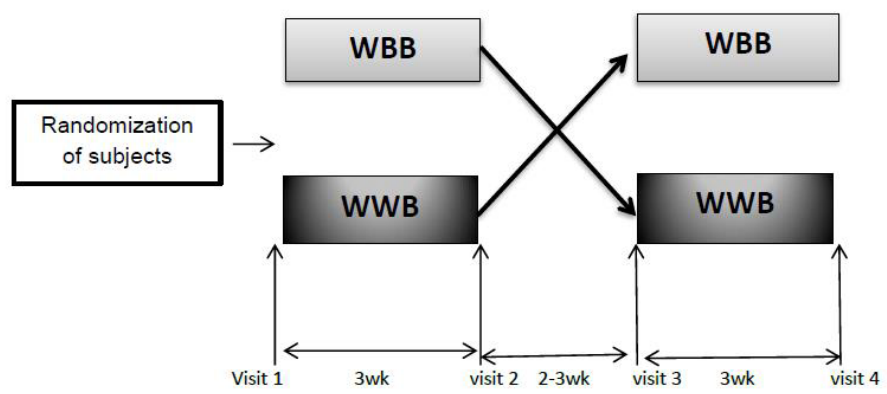
\includegraphics[scale=0.5]{studes}
    \caption{Schema of Study Design}
        \label{fig:studes}
\end{figure}

\subsection{\acrshort{cvd} Risk Factors and Other Health Status Indicators}
\acrfull{tc}, \acrfull{ldlc}, \acrfull{hdlc}, \acrfull{tg}, \acrfull{crp}, fasting glucose and fasting insulin were measured both before and after intervention. 

Besides \acrshort{cvd} risk factors, body weight and waist circumference were also measured. Urine and blood samples for this research were also collected during each visit. 

\subsection{Conclusions}
No significant effect of treatment was detected for \acrshort{tc} (p = 0.31), \acrlong{tg} (p = 0.11), CRP (p = 0.62), fasting insulin and glucose (p= 0.78 and 0.51, respectively), HDL–C and LDL–C (p = 0.32 and 0.25, respectively). 
This could be attributed to small sample size and short intervention period. In addition, the storage and food processing of bread could also affect the results\cite{Popovici2016}.

\section{Introduction}
\subsection{Barley}
\subsubsection{Barley in the farm}
Historically, barley (\textit{Hordeum vulgare}) has been an important cereal grain. It was among the first domesticated plants during the hundreds or thousands of years. It played an important role for human's transition from a hunting and gathering to agrarian lifestyle\cite{Baik2008,barleybook}. 

Nowadays, barley is one of the most produced grains in the farm. In 2016, 143 million tonnes barley were produced, ranked as 4th most produced grains, behind maize, rice and wheat. European Union countries produced 63\% barley of the world. Denmark produced 3.9 million tonnes barley in 2016 which was ranked as 11th most produced country of barley\cite{FAO2016}.

From the perspective of plant science, barley is arguably the most widely adapted cereal grain species with good drought, cold, and salt tolerance\cite{Ullrich2010}.
It is cultivated both in highly productive agricultural systems and also in marginal and subsistence environments\cite{barleyfeedtheworld}.
Barley's ability to adapt to multiple biotic and abiotic stresses\cite{barleyfeedtheworld} will be crucial to its future exploitation to deal with global food security issue.

\subsubsection{Barley on the table}
% table 
The status of barley on the table is incompatible with its large production 
in the farm. Barley for direct food use only remains important in few areas, e.g. Asia and northern Africa. Barley has been majorly used as a feed, malting and brewing grain\cite{barleyfeedtheworld,Baik2008}. About two-thirds were used for feed, one-third for malting and only about 2\% of total production were used for food directly\cite{Baik2008}.

Wheat and rice surpassed barley on the table, partially because wheat and rice products give a better mouth-feel and quality\cite{Baik2008}. Other reasons include relatively few efforts or attempts have been devoted to systematically breed and develop barley varieties for food uses, as well as food processing technique and product development\cite{Baik2008}. By far, the quality standard of barley for food use has not been well established, making it difficult for food manufacturers to select raw materials suitable for use in specific food products\cite{Baik2008}.

\subsubsection{Health Benefits of Whole Grain Barley}
Currently, research results of whole grain barley's health beneficial effects are still controversial. 

Some positive research results attributed barley's health benefit effects to its beta-glucan contents or rich phytochemicals. Barley contains 4.6\% beta-glucan by dry weight, while wheat, rye and oats contains 0.8\%, 1.5\% and 5.0\% respectively\cite{frolich2013whole}. Cereal beta-glucan was claimed to be capable of reducing blood serum cholesterol and regulating blood glucose levels\cite{frolich2013whole}. Some epidemiological studies also showed whole-grain cereals can protect against obesity, diabetes, \acrshort{cvd} and cancers\cite{Fardet2010}. Besides fibers of cereal, new hypothesis was also proposed that polyphenols, sulfur compounds, lignin and phytic acid, their antioxidant activities also contribute to barley's health benefit effects\cite{fardet2010}.

However, research results from University of Copenhagen showed that although beta-glucan of barley can induce satiety and reduce energy intake\cite{barleysatiety}, it did not affect cholesterol metabolism\cite{Ibrugger2013}. Barley's health beneficial effects and associated metabolic pathways still need further research results to achieve a clear conclusion.

A major problem underlying estimating barley's health benefit effects is lacking an objective measurement of its exposure. It will be further discussed in later text.
%Whole-grain wheat is also a rich source of methyl donors and lipotropes (methionine, betaine, choline, inositol and folates) that may be involved in cardiovascular and/or hepatic protection, lipid metabolism and DNA methylation\cite{fardet2010}.

%Potential protective effects of bound phenolic acids within the colon, of the B-complex vitamins on the nervous system and mental health, of oligosaccharides as prebiotics, of compounds associated with skeleton health, and of other compounds such as a-linolenic acid, policosanol, melatonin, phytosterols and para-aminobenzoic acid also deserve to be studied in more depth.\cite{fardet2010}

%High intake of whole grain cereal may benefit health in many aspects. This hypothesis has been under debate since long ago. Investigating relationship between specific food exposure and health status is important for nutritional study. However, measuring food exposure is normally based on subjects self-report1. It intrinsically consists bias and error. A potential way to avoid bias and error is by measuring food intake biomarker in subjects biological fluids1. 
%Biomarkers for whole grain intake has been widely used as a method to assess the intake. Alkylresorcinol in plasma and urine has been proved as intake biomarker for whole grain wheat and rye2. However, barley, the 4th most produced cereal in the world lacks the discovery of intake biomarker.
%Previous clinical research tested whole grain barley intervention on cardiovascular disease (CVD) as a comparison with whole grain wheat. However, no significant evidence can prove whole grain barley is able to relief CVD risk factor.

\subsubsection{Renewd Interest of Barley in Food Industry}
In the past decades, barley has attracted a lot of interest of food producers and consumers to be used as a healthy food ingredient\cite{Baik2008}, especially in baking industry\cite{Sullivan2013}.

Renewed interest of barley for food uses largely centres around the effects of beta-glucans on lowering blood cholesterol levels and glycemic index. In addition, whole grain barley foods were considered to be capable of increasing satiety, reducing energy intake and weight loss\cite{Baik2008}.

There is a great potential for food industry to develop barley-based healthy food as a substitute for popularly used cereal grains such as wheat, oat, rice, and maize\cite{Baik2008}.

\subsection{Whole Grain Cereal Intake Biomarkers}
\subsubsection{\acrfull{bfis}}
The research interests and tasks of modern nutrition science have shifted gradually these years \cite{Scalbert2014}. Especially in developed or newly-developed countries, e.g. Denmark and China, nutrition associated diseases trends from essential nutrients deficiency disease to chronic diseases, e.g. obesity, diabetes, \acrshort{cvd} and cancer. The research objects also changed from 7 types of essential nutrients to a large group of non-essential nutrients. It attracts increasing interest to research non-essential nutrients' health benefit effects, chronic disease prevention effects, their metabolic and signaling pathways etc.

This trend in nutrition science reseach also raised a question, 'how to accurately, objectively and economically measure the intake of these non-essential nutrients?' By far, the application of \acrfull{bfis} has been proven that it can provide a more objective method to measure dietary exposures with a high precision and detail\cite{Scalbert2014}.

Dietary exposure has traditionally been measured by self-reported methods, e.g. 24-hour dietary recalls or food-frequency questionnaires\cite{Rutishauser2005DietaryMeasurements.}. 
However, these methods consist a lot of subjective factors, such as recall bias and difficulty in assessing portion sizes\cite{Scalbert2014}. 
Additionally, such as cigarettes and alcohol consumption could also be biased by self-reporting methods because of cultural and societal attitudes towards these consumptions. 
Hence, these self-reporting methods intrinsically consist bias and errors.

The wrongly-estimated dietary exposure will further affect the study results of correlations between dietary exposures and disease frequencies, drawing controversial or even wrong conclusions\cite{Scalbert2014}.

\subsubsection{Alkylresorcinols}
Alkylresorcinols and their metabolites can be used as whole grain cereal intake biomarkers.
It was reported and validated in around a dozen of researches both in intervention study and population study, shown in the table.
Alkylresorcinols and their metabolites can be detected both in urinary and plasma samples.

However, vast majority of these studies mentioned above were focused on whole grain wheat or rye, or taking into account of whole grain cereals group. By far, there exists no biomarker specifically to indicate barley intakes.

%\newgeometry{landscape}

%\begin{landscape}
\begin{center}
\scalebox{0.6}
{
\begin{small}


\begin{tabular}{|m{0.5cm}|m{1.8cm}|m{2.5cm}|m{2.5cm}|m{2.5cm}|m{2cm}|m{2cm}|m{2cm}|m{0.8cm}|m{0.3cm}}
%\begin{tabu} to 1.2\textwidth { | c | c |X[c]| X[c]| X[c]| X[c]| X[c]|c| c| c}
 \hline
No & Authors & Experimental\newline methods & Food types & Compounds & Subjects & Matrix & Reference\\ \hline
1&	Wierzbicka, R etc.&	three-day weighed food record &	Whole grain cereals	&alkylresorcinol metabolites	& 69 Swedish	& urine &	\cite{ISI:000404730400012}\\ \hline
2&	Zhu, YD etc.&Diet Intervention&Whole grain wheat&alkylresorcinol metabolites,
benzoxazinoid derivatives,phenolic acid derivatives&12 healthy participants&urine&	\cite{ISI:000387249200001}\\ \hline
3&	Garcia-Aloy, M etc.&	Self-reported food frequency questionnaires&	whole grain bread	&phytochemicals (benzoxazinoids, alkylresorcinol metabolites) &	155 subjects	&urine	&\cite{ISI:000384784900008}\\ \hline
4&	Magnusdottir, OK etc.&	controlled diet&whole grain rye&	alkylresorcinol C17:0/C21:0 ratio&	93 metabolic syndrome patients in Nordic countries&	plasma&	\cite{ISI:000343662800061}\\ \hline
5&	Lappi, J etc.&	Diet Intervention&	whole grain and fibre riched rye bread&	alkylrecorsinol& &		plasma	&\cite{Sawicki2016}\\ \hline
6&	Ma, JT etc.	&Self-reported food frequency questionnaires&	whole grain cereals&	alkylrecorsinol&	407 olders	&plasma&	\cite{ISI:000309032000011}\\ \hline
7&	Ross, AB etc.&	Diet Intervention&	whole grain food (including wheat, oats, brown basmati rice, corn, rice, barley)&alkylrecorsinol&	316 overweight and obese participants&	plasma&	\cite{ISI:000298402100026}\\ \hline
8&	Andersson, A etc.&	Food records&	whole grain wheat and rye&	alkylrecorsinol&	72 Swedish adults&	nonfasting and fasting plasma&	\cite{ISI:000294523500019}\\ \hline
9&	Landberg, R etc. &	semi-quantitative food frequency questionnaires&	rye bread&	alkylrecorsinol&	360 post-menopausal women&	plasma&	\cite{Landberg2009}\\ \hline
10&	Montonen, J. etc.&	Self-reported food frequency questionnaires&	Whole grain food&	alkylrecorsinol&	100 healthy adults&	plasma	&\cite{ISI:000279623300007}\\ \hline
11&	Guyman, LA etc.&	three-day food record and food frequency questionnaires&	Whole grain food&	3-(3,5-dihydroxyphenyl)-1-propanoic acid& &	urine&	\cite{ISI:000259554500019}\\ \hline
12&	Landberg, R etc.&	Diet Intervention&	whole grain wheat and rye&	alkylrecorsinol&	22 women and 8 men&	plasma	&\cite{ISI:000255012000007}\\ \hline
%\end{tabu}
\end{tabular}
\end{small}
}
\end{center}

\subsection{Novel Dietary Biomarkers Identification by Untargetted \\ Metabolomics}
\subsubsection{Metabolome Profiling Techniques}
With the development of high-throughout analytical technologies, 3 techniques has been majorly used in untargetted metabolomics study to identify novel dietary biomarkers. They are \acrfull{lc/ms}, \\\acrfull{gc/ms} and \acrfull{nmr} \cite{Scalbert2014}. 

The detailed comparisons of these techniques are out of this project scope. But, within these 3 techniques, \acrshort{lc/ms} has an outstanding role and is briefly described:

It has been proven with the advantages of:

(1) high sensitivities: the low detection limit allows tiny amount of metabolites detection.

(2) wide coverages of analytes: abundant commercially available columns, different mobile phase combination, gradient elution and temperature etc. can be optimized to adapt to different analytical tasks.

However, compared its omic-cousins, metabolomics is still not a global technique. Not all metabolites can be profiled in a single analysis.

\subsubsection{Metabolomics data analysis}
Metabolomics data analysis generally consists data preprocessing, data alignment, data normalization and signal correction followed by the analysis through various statistical methods \cite{Scalbert2014}

\subsubsection{Compound Identification and Validation}
Compound identification has been recognized as the most difficult aspect hurdling the discovery of novel biomarkers. Not only limited to \acrshort{bfis}, compound identification troubles almost all Metabolomics researches, including disease diagnose biomarkers etc.

In the 1st Copenhagen Clinical Metabolomics Conference held in Hellerup, Denmark on 25-26 Oct 2018, experts from diverse Metabolomics research areas proposed several insightful suggestions that currently or in the future could impact the methods for compound identifications. These orally presented proposals were summarized as following:

\begin{itemize}
    \item \textbf{Improvement of analytical instruments for metabolome profiling:} as proposed by Karolina\footnote{Karolina Sulek, Novo Nordish Foundation Center for Protein Research, University of Copenhagen, Denmark}, the signals of biomarkers could be very low and the detection can easily be interfered by noise or other compounds in metabolome profiling. 
    
    The development of novel analytical instruments could increase analytes coverage or increased resolving power which may have an impact on compound identification in the future.
    
    For example, \acrfull{tims-pasef} can profile metabolome with high resolution generating a 4-dimentional dataset (ion mobility, retention time, mass to charge ratio and intensity). The unique 4-D fingerprint can make compounds identification easier.
    
    \item \textbf{Bioinformatics, database and data sharing:} as proposed by Cristina\footnote{Cristina Legido-Quigley, Steno Diabetes Center, Denmark}, Gabi\footnote{Gabi Kastenmüller, HelmholtzZentrum München, Denmark}, David\footnote{David Wishart, University of Albertaz, Canada}, Niles\footnote{Nils Færgeman, University of Southern Denmark, Denmark} and Pieter\footnotemark, compound identification could be revolutionized by using bioinformatics such as computational chemistry to predict MS/MS spectra of metabolites. Then these data can be shared via database such as\acrfull{hmdb} \cite{hmdb} and be accessible by the whole community.
    
    Pieter\footnotemark[\value{footnote}] also pointed out a lot of spectra were generated but not open to the community. \footnotetext{Pieter Dorrestein, University of California San Diego, USA}He proposed that metabolomics researchers should share \acrshort{ms/ms} spectra in \acrfull{gnps} \cite{GNPS}. These spectra can be accessed by the whole community. In addition, a computer algorithm namely 'molecular network' can calculate the similarities between unknown compounds and annotated compounds in the database. Hence, researchers can get annotation suggestions of unknown compounds. 
    
    \item \textbf {Deepening the understanding of biological aspect of metabolism:}     Marta\footnote{Marta Cascante, University of Barcelona, Spain} proposed that, the technical aspect of metabolomics is relatively mature, such as analytical instruments and bioinformatic tools. On contray, the real bottleneck limiting deeper understanding of metabolomics is its biological aspect. If we can deepen the understanding of it biological aspects (such as signaling, metabolic pathway etc.), we can better understand metabolomics itself in return. Therefore, the compound identification could be easier.
 
    \item \textbf{'Correctly' identify the identifiable compounds:}
    Mesut\footnote{Mesut Bilgin, Danish Cancer Society, Denmark} is an expert in shotgun mass spectrometry based lipidomics.
    He proposed a unique perspective for compound identification but could be inspiring. 
    
    He pointed out that, unlike its omic counsins, identifying all metabolites is currently impossible in metabolomics research. Therefore, it is important to 'correctly' identify those identifiable compounds. 
    
     A systematic protocol for mammalian lipidome analysis has been built up by him and his colleagues\cite{Nielsen2017}. The key ideas were briefly summarized as following: 
     
     An extensive in-house database was built covering all 'biologically-feasible' lipids based on their chain length and unsaturation degree. In addition, he emphasized a strict analytical conditions. For example, the lipid extraction should always be conducted under 4 degree to avoid plastic dissolving into the organic solvents. 
     By the way, based on a lot of preliminary experiments, he chose specific brands of solvents, plastic containers, experimental temperature etc to avoid contaminants to the maximum extent. Further, he sticked strictly to these conditions. Therefore, it can reach a correct identification as well as quantification.
\end{itemize}

Besides these proposals from experts, compound identification, especially for \acrlong{bfis} discovery, identification also relies on the knowledge or progress from other disciplines, such as food chemistry, plant science. A systematic literature research is suggested to 'dig' information for compound identification\cite{Pratico2018}.

%\textbf{Hypothesis}
%Some biomarkers can indicate barley intake in urine sample based on untargeted metabolomics. 

%\textbf{Methods}
%Urine sample was analysed by LC-MS. 
%LC-MS Data will be pre-processed by MZmine through the step: 
%noise filtering, baseline correction, peak detection, deconvolution, alignment and normalization.

%After pre-processing, 
%multivariable data analysis (PCA and PLSDA) 
%by PLS toolbox will clue the potential features for later identification. In the end, potential compounds will be identified using databases as reference. MS/MS can also be used to verify the identification results.

%\textbf{Result}
%X, X, X can be whole grain barley intake biomarker.

\section{Materials and Methods}
\subsection{Chemicals}
80\% ethanol (CAS 64-17-5,96\%, diluted by MiliQ water), solvent A (miliQ water + 0.1\% formic acid), solvent B (0.1\% formic acid in 70\% acetonitrile and 30\% methanol)

\subsection{Apparatus}
Rotational vacuum concentrator (RVC 2-35, Martin Christ, Germany), 
kitchen high speed blender, ultrasonic bath (Branson 3800), vortex mixer, centrifuge.

Two sets of \acrfull{lc/ms} systems were used: 

UPLC-QToF: An ultraperformance liquid chromatography (UPLC) system coupled to a quadrupole time-of-flight mass spectrometer (Premier QTOF, Waters Corporation, Manchester, UK) was used for urine sample analysis.

UPLC-Vion QoF: An ultraperformance liquid chromatography (UPLC) system coupled to Vion IMS QTof Ion Mobility Quadrupole Time-of-flight Mass Spectrometry, Waters, USA)

More details regarding \acrshort{lc/ms} analytical condition can be found elsewhere\cite{Jensen2016,Barri2012MetabolicCoverage.}

\subsection{Whole Grain Barley}
Whole grain barley cereal (1.5 kg, Aurion, Denmark) was purchased from Helsehuset, Gammel Kongevej 92, Frederiksberg.
%Whole grain wheat flour (1 kg, Finax, Denmark) was purchased from Føtex, Frederiksberg.
Whole grain barley was first grained by a high-speed kitchen blender and then filtered by a sieve (2 mm * 2 mm). Two fractions were achieved after sieve filtration. 

The fraction that can pass through the sieve had smaller particle size (smaller than 2 mm). This fraction demonstrated light brown colour and majorly came from barley outer layer, i.e. bran part.

The other fraction had bigger particle size. This fraction demonstrated white colour, but containing sparsely-distributed light brown particles. This fraction majorly came from inner barley, i.e. endosperm part. They were further smashed by a mortar and filtered by the sieve (2 mm * 2mm).

\subsection{\acrshort{lc/ms} Analysis of Urine samples and Whole Grain Barley}
%urine
Urine samples were collected 24 hours after intake of test bread. Samples were diluted 10 times by MiliQ-water then stored in -80 \degree C until analysis. The metabolome was profiled by UPLC-QTof, together with internal standard, metabolomics standard and pooled samples. 
%blood samples were drawn by a trained bio analyst from each participant at 4 different time points: at the beginning and at the end of each intervention period (visit 1–baseline, visit 2–week 3, visit 3– week5, visit 4– week–8)

%extraction
Whole grain barley powders were extracted by 80\% ethanol twice. The ratio (v/m) between ethanol and barley was 0.015, i.e. 15 mL per gram. Each extraction session lasted 30 min with the assistance of ultrasonic in room temperature. The supernatants were collected after 1st extraction session. Then, fresh ethanol solution were added to start 2nd extraction session. In the end of the extraction, supernatants from both sessions were combined in brown bottles. 2 mL supernatants from each bottle were further transferred to eppendorf tubes. Solvents in eppendorf tubes were evaporated by a rotational vacuum concentrator overnight.

Outer layer and inner powders were treated separately. Both of them were extracted in triplicates. The extraction was conducted in a yellow light room. All glasswares and eppendorf tubes were brown or covered by aluminium foils to protect light sensitive extracts.

%prepare for injection
\SI{200}{\micro\liter} solvent A was used to reconstitute the extracts. Further they were diluted 10-fold to avoid ion suppression. The samples were centrifuged and the supernatants were transferred into vials for injection.

\subsection{Data Preprocessing} 
    % Data convertion
    Raw data was first converted into '.cdf' format by DataBridge, an \acrshort{lc/ms} data file conversion program built-in MassLynx developed by Waters company.
    
    % MZmine step
    Then, data was preprocessed by MZmine (v2.31) following the steps: peak detection, deisotoping, alignment and gap filling.
    Positive mode and negative were separately processed because of different noise level and in-source reaction.
    
    % result
    In the end, the detected features, including information of mass to charge ratio (m/z), retention time (rt) and intensities were output as '.csv' files for further investigation.
    
\subsection{Data Analysis and Variable Selections}
Data analysis was performed in MATLAB R2018a (v9.4.0.813654). 
Data was analyzed by \acrfull{pca}, \acrfull{plsda} and cross validation in PLS\_Toolbox (v8.6.2, Eigenvector Research Inc).

Further, potential biomarkers were selected for identification, which will be described in later texts.

%PCA
    \acrshort{pca} analysis is a unsupervised multivariable statistical method. Multivariate analysis is most commonly used for exploratory analysis of metabolome profiling data \cite{Worley2013UtilitiesPlots.}. It was often considered as starting point to analyze metabolome profiling data \cite{Scalbert2014}. Becaues \acrshort{pca} can provide an objective assessment of the principal patterns in the data set (e.g. intake or non-intake)\cite{Scalbert2014}. \acrshort{pca} can also detect outliers to control the data quality\cite{gurdenizdata}.
    
    For both modes, \acrshort{pca} modeling used autoscale and \acrfull{pqn} as preprocessing methods.
    
%PLSDA modeling
    \acrshort{plsda} is the most commonly used supervised multivariable analysis\cite{Scalbert2014}. 
    \acrshort{plsda} was used to differentiate the barley and wheat intake.
    
    Variable were selected by repeatedly removing variables with selectivity ratio and \acrfull{vip} values lower than 1 until no further increase in the cross-validation classification errors could be observed.Final models with selected variables were evaluated using test set misclassification. The variables that were selected in at least 75\% of the models were recorded for further investigation.
    
%Variable selections
    Potential barley intake biomarkers were selected from these variables based on the criterials:
    \begin{itemize}

        \item They should have low intensities in group \acrfull{bb}, \acrfull{bw}, \acrfull{aw}
        \item They should have high intensities in intervention group \acrfull{ab}
    \end{itemize}


 
\subsection{\acrfull{ms/ms} Experiment and Identification}
    %How do I know which peak is molecular ion?
\acrfull{ms/ms} can select specific ions of interest and fragment them. \acrshort{ms/ms} is an important method in structure elucidation. \acrshort{ms/ms} was performed by Vion. Collision energy of 14 ev, 28 eV, 42 eV were used to achieve different extent of fragmentation. Database HMDB, m/z cloud and Chemspider were used. MS/MS spectrum was also input into SIRIUS (version 4.0.1, build 3) to predict the structure.

    


\section{Results}
\subsection{\acrshort{lc/ms} Analysis of Whole Grain Barley}
The elution patterns of barley flour chromatograms (shown in Appendix) were mostly similar. Elution time of several peaks slightly deviated, but all within 0.02 min.

However, one major difference of the chromatograms was, bran powder had higher intensities than endosperm powders for some peaks. For example, in negative mode, bran powder had double intensities for peaks with retention time (min) 3.84, 3.97, 4.43 compared with endosperm powder.
The large difference could be explained by bran powder containing more 'whole grain' part. The compound in this part was more soluble in ethanol. But errors originated from the extraction was also possible.

\subsection{Data-preprocess}
After data-preprocessing, 1719 features were detected in positive mode; in negative mode, 3304 features were detected. 
Based on previous experience, it was very common to observe that more features were detected in negative mode than positive mode.

It could be explained by, either the instrument performs better in negative mode having a higher resolving power, or, some metabolites could be ionized easier in negative mode than positive mode, e.g. glucuronate conjugates.

\subsection{\acrshort{pca} Modeling}
%PCA
\acrshort{pca} modeling results were shown in Figure \ref{fig:pca}. In score plot, \acrfull{aw} and \acrfull{ab} can not be well separated. 

\acrshort{pca} can also detect outliers and be used for data quality control\cite{Scalbert2014}. 
In both modes, pooled samples located tightly near the center, which indicated that the data had a high quality. 
Two subjects were detected as outliers (outside 95\% confidence level limit) in both modes. 
We investigated raw data and observed that these two subjects almost showed high intensities in all variables. 
The reason could be their urine samples were too concentrated.

This is why metabolomics research could be very complex.
Although subjects were treated with the same intervention and biofluids were collected, processed and analyzed in the same way. But the metabolome could vary a lot between individuals.
Unlike laboratory animals, humans are free-living individuals. Metabolome could be affected by a lot of external factors, such as genes, living environments and health statues.

In this case, concentrated urine could be simply attributed to that these individuals did not drink enough water. These two subjects were not removed in further study.
\begin{figure}[h]
    \centering
    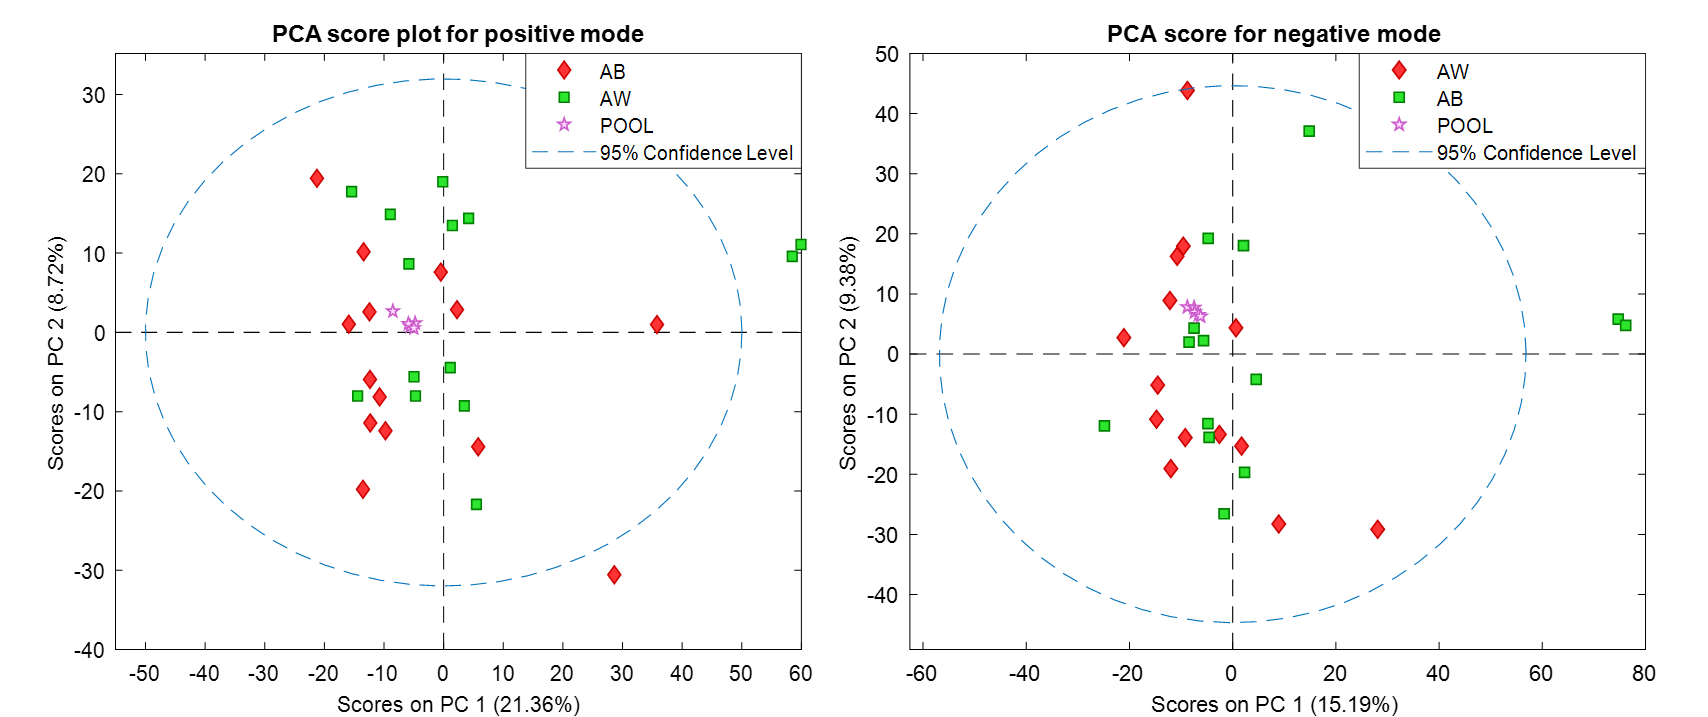
\includegraphics[scale=0.43]{images/pca_score.png}
    \caption{PCA score plot (AW= After Wheat, AB= After Barley, POOL= pooled samples)}
    \label{fig:pca}
\end{figure}

\subsection{\acrshort{plsda} Modeling and Variable Selections}
%PLSDA
\acrshort{plsda} modeling selected 72 variables out of 1719 features in positive mode; 86 variables out of 3304 features in negative mode.  These selected variables had high \acrshort{vip} value and selectivity ratio.

Although they can differentiate barley and wheat intake, not all of them were classified as potential biomarkers for barley intake. 
\begin{figure}[h]
    \centering
    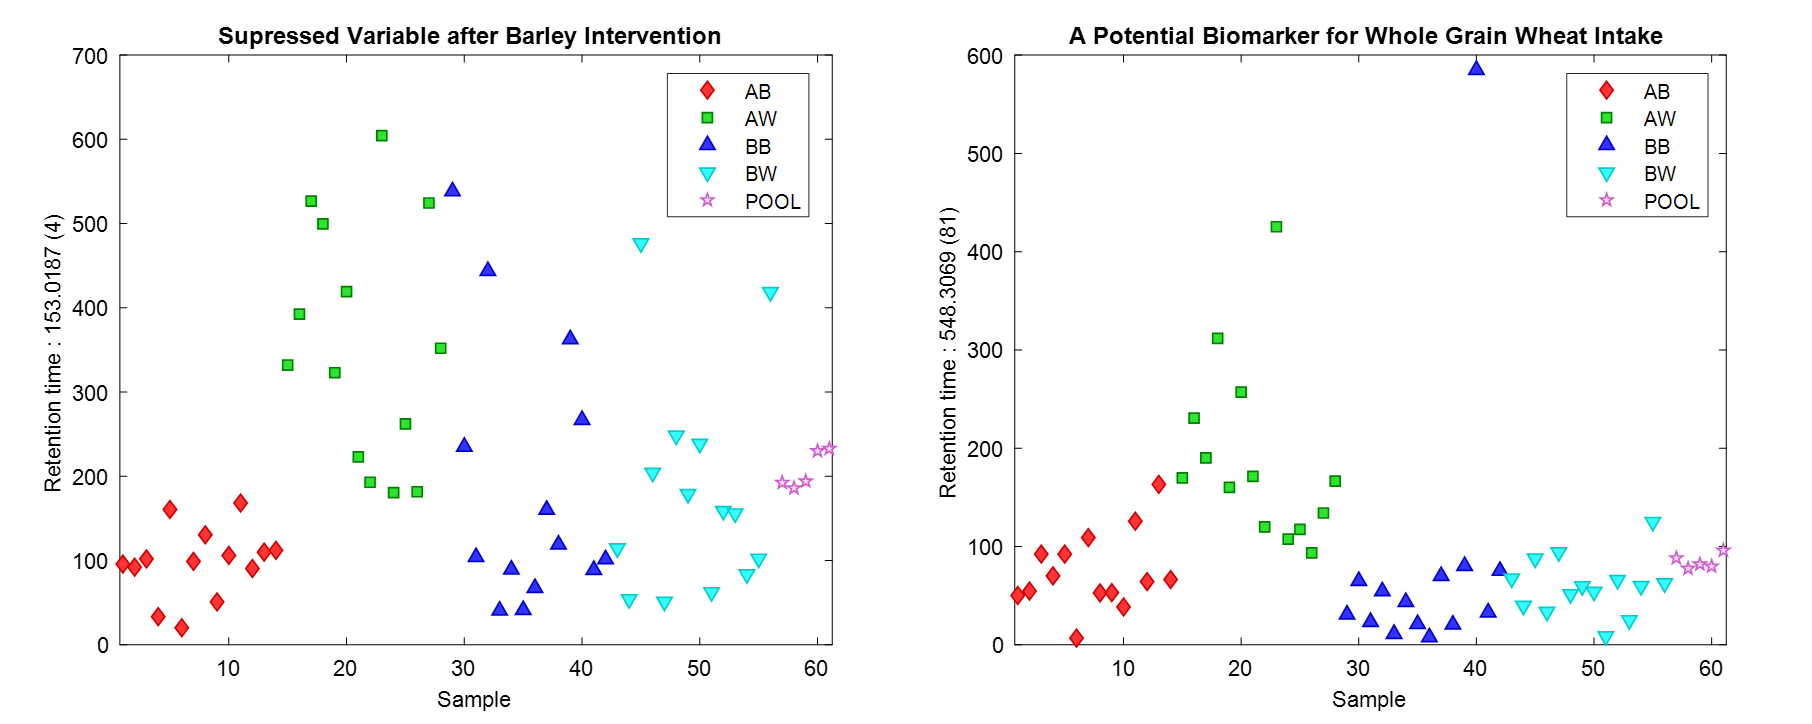
\includegraphics[scale=0.36]{images/marker1.png}
    \caption{Variables Selected by PLSDA modeling but not classified as potential barley intake biomarkers (AW= After Wheat, AB= After Barley, POOL= pooled samples)}
    \label{fig:marker1}
\end{figure}
\begin{figure}[H]
    \centering
    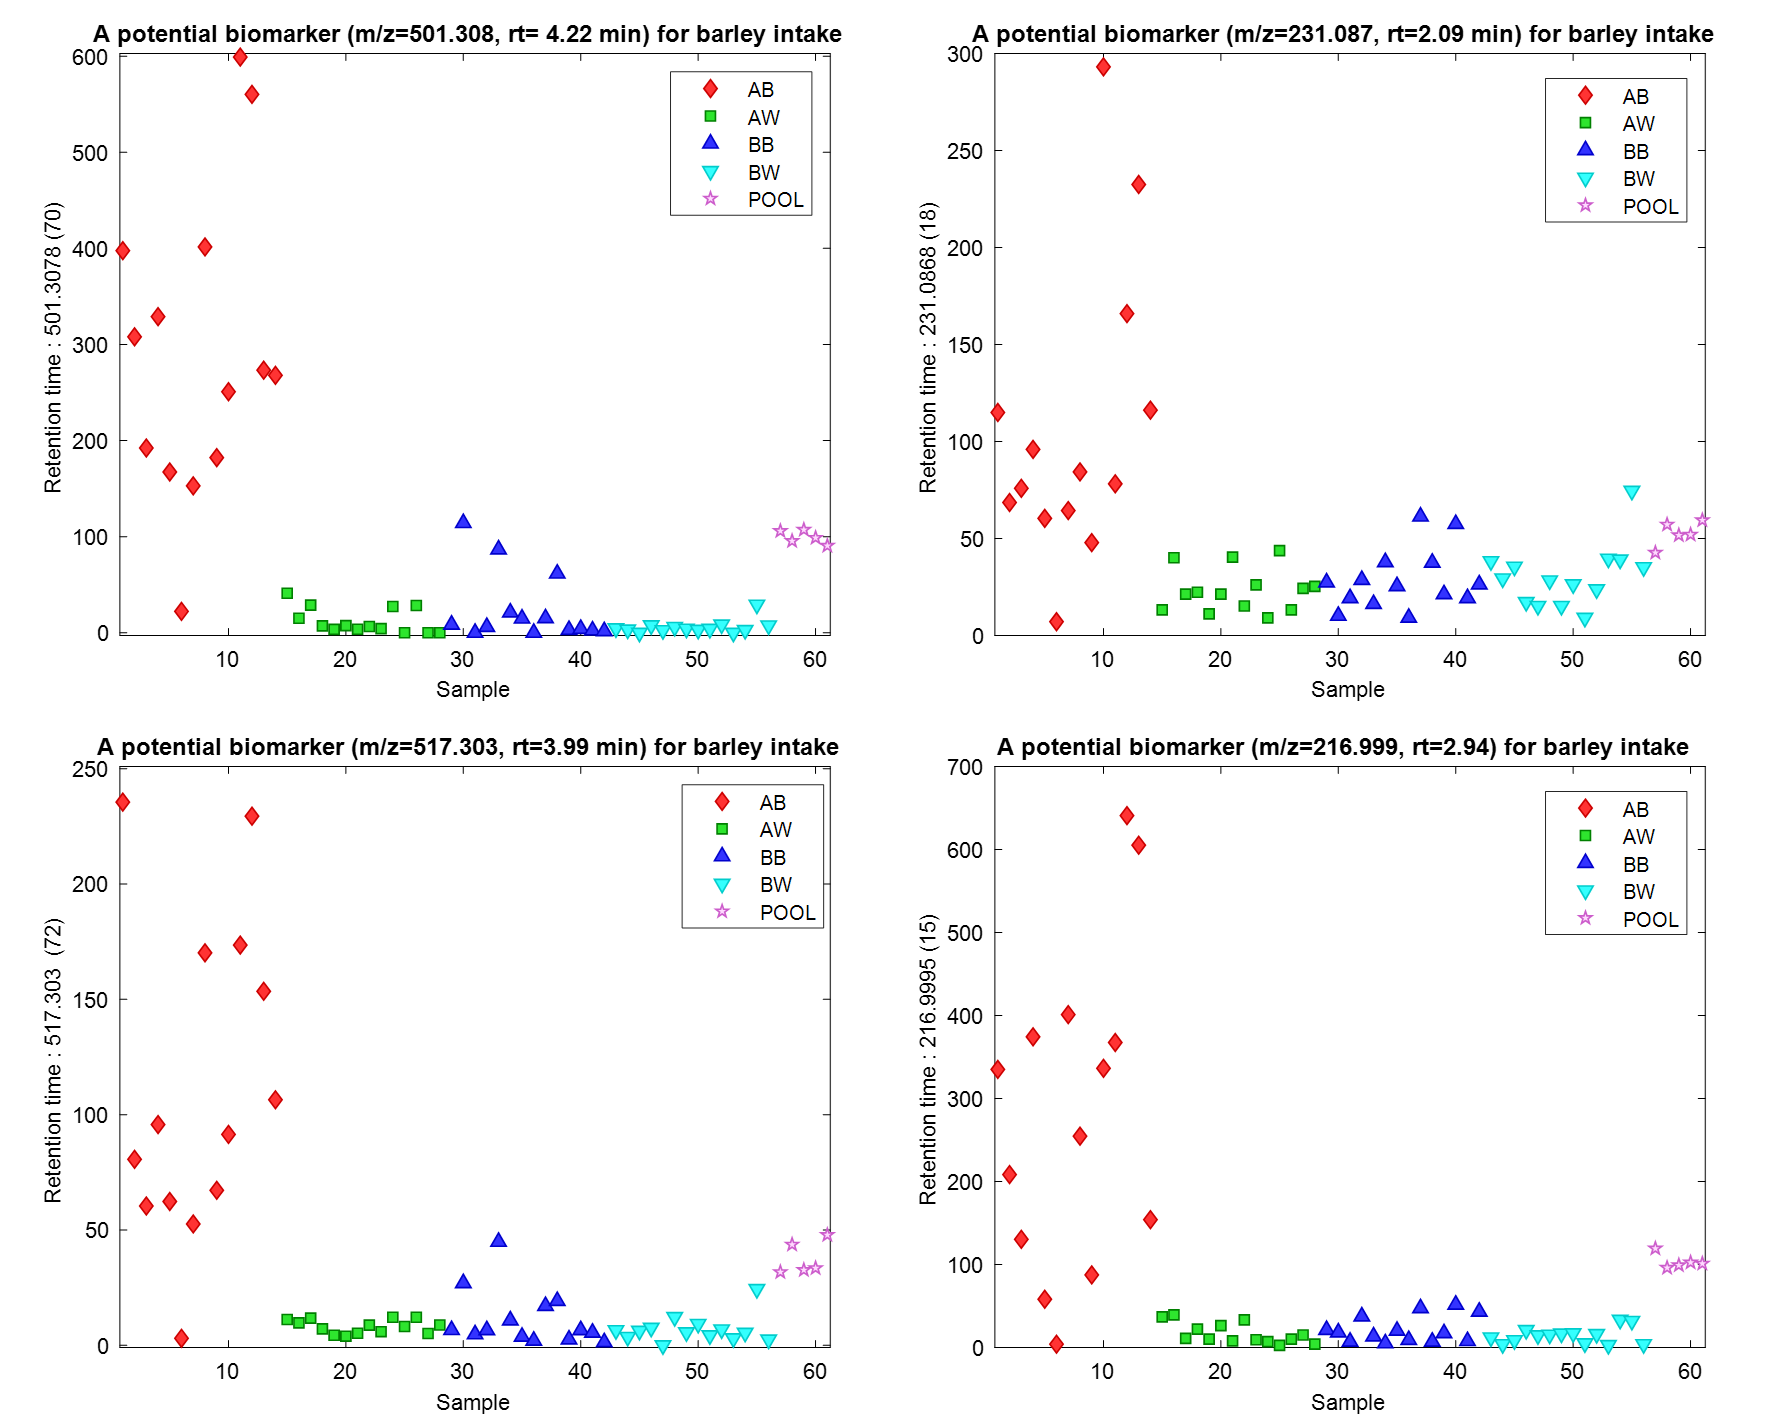
\includegraphics[scale=0.36]{images/barley_marker.png}
    \caption{Intensity differences of potential barley intake biomarkers in different intervention time-points (AW= After Wheat, AB= After Barley, POOL= pooled samples)}
    \label{fig:selected}
\end{figure}
\clearpage
For example, as shown in Figure \ref{fig:marker1} (left), the intensity of this variable got suppressed after barley intake. This could be an endogenous metabolite suppressed by barley intake. In Figure \ref{fig:marker1} (right), this variable could be a potential biomarker for whole grain wheat intake. Because it had lower value in \acrshort{ab}, \acrshort{bb}, \acrshort{bw} but increased intensities after whole grain wheat intake.

%Potential biomarkers selection
Potential biomarkers for barley intake were further selected based on the criterials as described before to perform \acrshort{ms/ms} analysis for identification. Within these potential biomarkers, 5 were from negative mode and 1 was from positive mode. Figure \ref{fig:selected} showed intensities of biomarkers (part) in different time-points before and after intervention.

\subsection{\acrfull{ms/ms} and Identification of Potential Biomarkers}
\subsubsection{m/z 231.0870}
This ion was detected in negative mode. Intensity of this ion was too low to be detected in \acrshort{ms/ms}. Moreover, there was no feasible hints in the database. Possible formulas were summarized in Figure \ref{fig:231p0870}.
\begin{figure}[h]
    \centering
    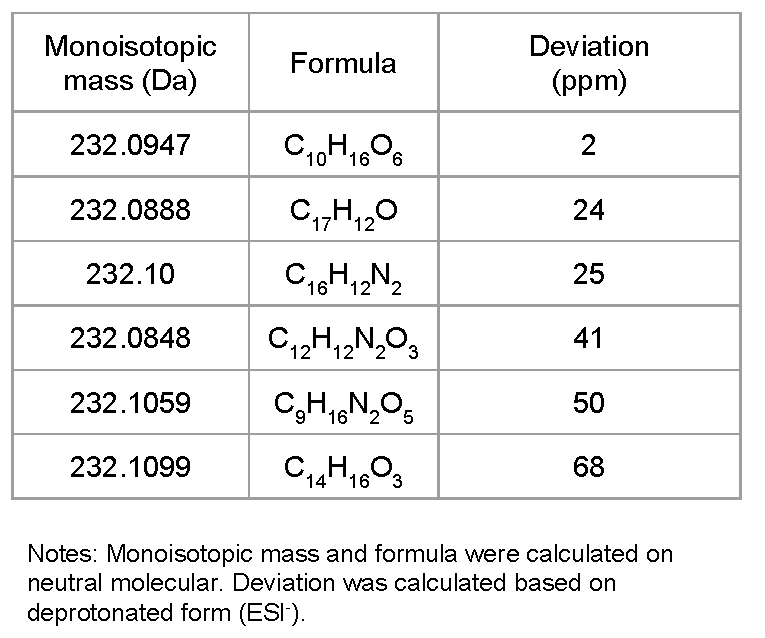
\includegraphics[scale=0.5]{images/231p0870.pdf}
    \caption{Possible formulas of ion m/z 231.0870}
    \label{fig:231p0870}
\end{figure}

\subsubsection{m/z 775.3401}
This ion was detected in negative mode. It was annotated as the dimer of [C\textsubscript{18}H\textsubscript{28}O\textsubscript{9}-H]\textsuperscript{-} with neutral mass 388.1735. However, the intensities of both monomer and dimer were too low to be detected in \acrshort{ms/ms}. No feasible hints existed in the database.

\subsubsection{m/z 216.9995 - phenol or polyphenol metabolite}
This ion was detected in negative mode. 
\begin{figure}[h!]
    \centering
    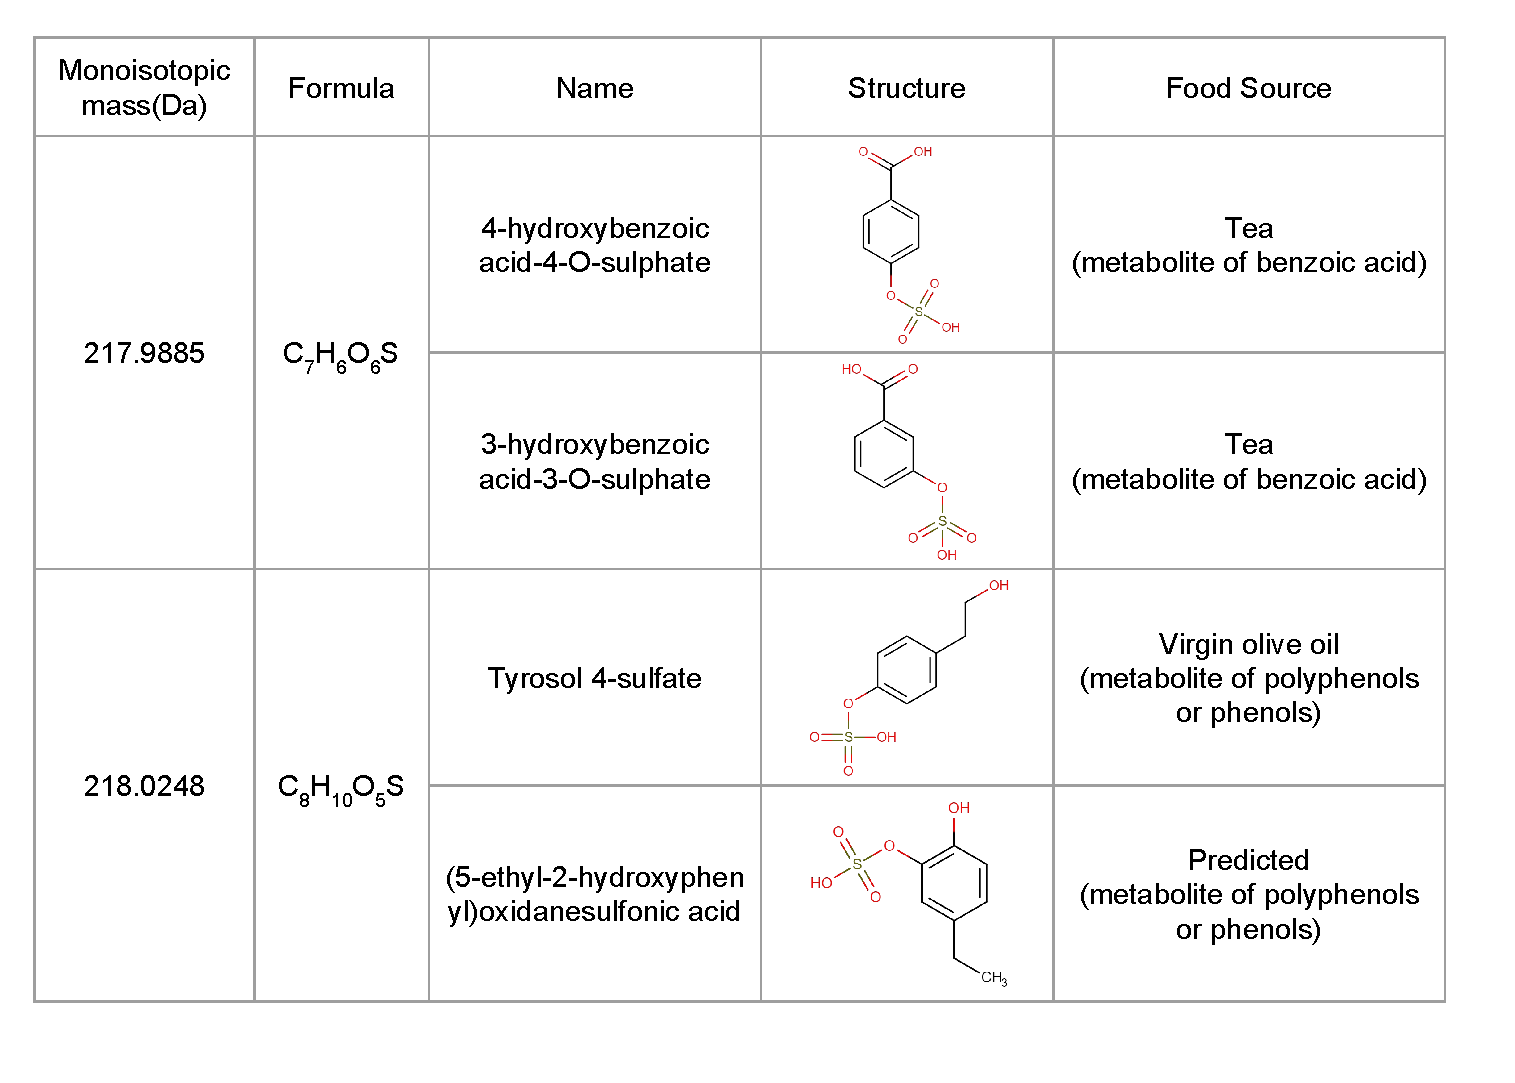
\includegraphics[scale=0.46]{images/216d9995.pdf}
    \caption{Possible structures of ion m/z 216.9995}
    \label{fig:216p9995}
\end{figure}
Although this potential biomarker can distinguish barley and wheat intake, the intensity of this ion was too low to be detected in \acrshort{ms/ms}. In addition, this ion was not detected in barley samples. The reason could be either it was not ionized or it was bio-transferred. 

From HMDB database\cite{hmdb}, several feasible compounds matched its mass. Figure \ref{fig:216p9995} summarized the feasible structures. These compounds were all either detected or predicted metabolites of polyphenols, phenols and bezoic acids.

4-hydroxybenzoic acid-4-O-sulphate and 3-hydroxybenzoic acid-3-O-sulphate were isomers and had the same formula, C\textsubscript{7}H\textsubscript{6}O\textsubscript{6}S. They were both detected in urine after tea intake and identified as benozic acid metabolites\cite{tea}.

Tyrosol 4-sulfate was detected in plasma after virgin olive oil intake and identified as metabolite of polyphenols or phenols\cite{oliveoil}. (5-ethyl-2-hydroxyphenyl) oxidanesulfonic acid was a predicted metabolite of polyphnols or phenols\cite{polyphenolphd}.

Because whole grain barley is rich in phenols, polyphenols and benzoic acids \cite{Idehen2017}. Meanwhile, sulfidation is a common phase II metabolic reaction\cite{phase2}. These compounds could also present in the urine after barley intake.

Although whole grain wheat also contains polyphenols, different concentration, structure or metabolic pathways could be the reason why barley and wheat intake can be distinguished by these compounds. This proposal needs to be further validated.

\subsubsection{m/z 517.3030 and 501.3080 - glucuronide conjugates}
These two potential biomarkers were detected in negative mode. 
Their neutral molecular formulas were differentiated by an oxygen atom, C\textsubscript{30}H\textsubscript{46}O\textsubscript{7} and C\textsubscript{30}H\textsubscript{46}O\textsubscript{6}.
They were putatively identified as glucuronide conjugates of barley metabolites.

\acrshort{ms/ms} spectra (Figure \ref{fig:501517compare}) showed a highly-similar pattern between m/z 50-200. A characteristic lost  (-176) of glucuronide conjugates\cite{phase2} was detected for both ions. The un-conjugated ions (341.26754, 325.27394) were detected as well. However, un-conjugated ions were not detected in barly in both modes. Either they were not ionized, or they were bio-transformed.
\begin{figure}[h]
    \centering
    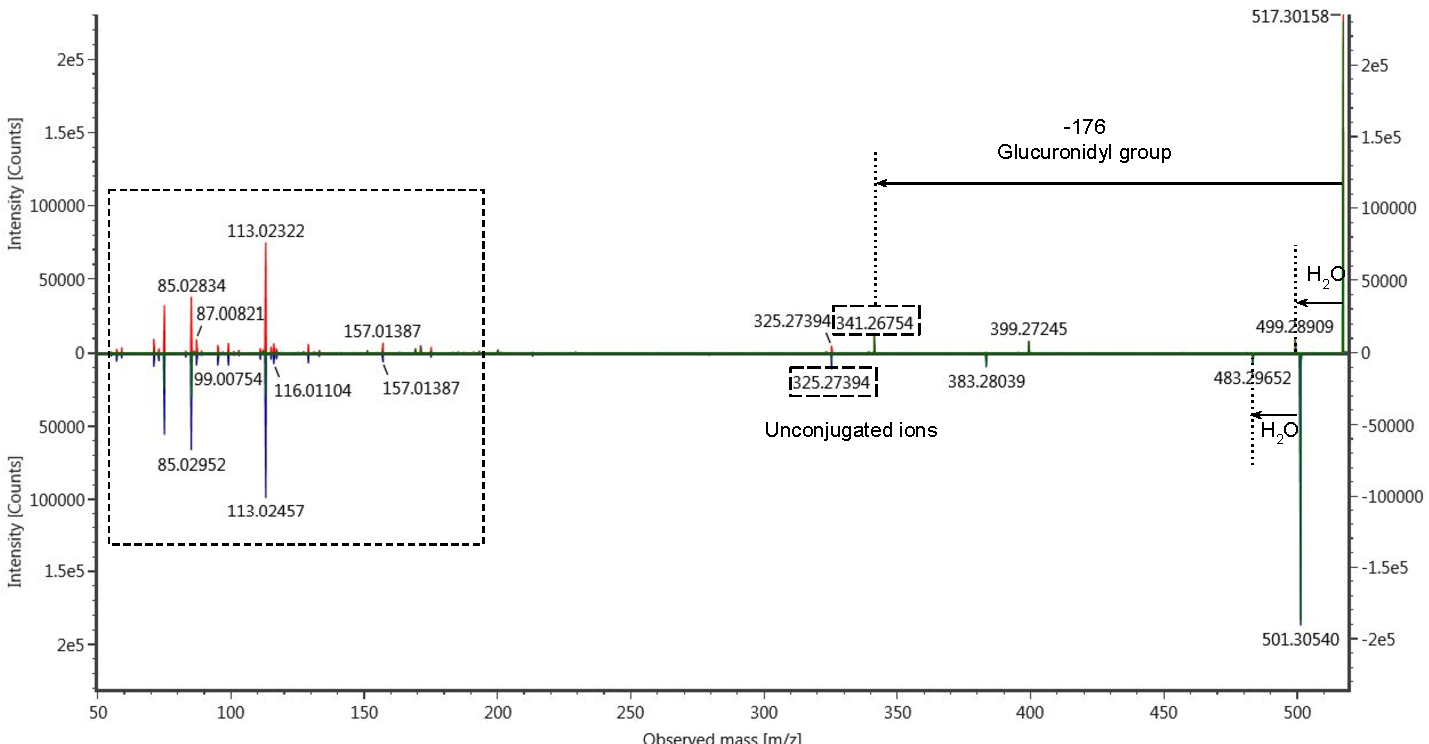
\includegraphics[scale=0.5]{images/501517compare.pdf}
    \caption{MS/MS spectra of ion(m/z=501 and 517) in urine sample, collision energy=42 eV}
    \label{fig:501517compare}
\end{figure}

In low mass region (m/z 50-200), it was difficult to differentiate the origins of fragments were from glucuronic acid or from un-conjugated molecular. Secondary fragments of glycuronyl moiety  (Figure \ref{fig:gluco_frag.PNG}, adapted from \cite{phase2}) interferred the identification.
\begin{figure}[h!]
    \centering
    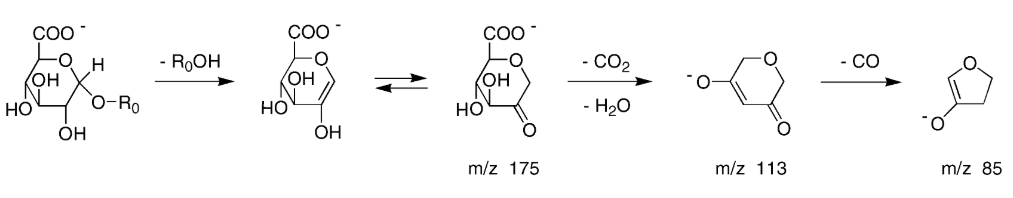
\includegraphics[scale=0.45]{images/gluco_frag.PNG}
    \caption{Secondary fragmentation of the glycuronyl moiety in negative-ion MS/MS spectra of glucuronide conjugates.}
    \label{fig:gluco_frag.PNG}
\end{figure}
% However, their detailed structures has not been clearly determined yet in this study.

% glucuronic acid reaction
Conjugation reactions with glucuronic acid occur in animals with glucuronosyltransferase after activation of the acid to uridine-5'-diphosphate glucuronic acid (UDP-5'- glucuronic acid). The glucuronic acid is bound to the corresponding molecule by a glycosidic linkage\cite{phase2}.
Besides glucuronide conjugates, glucosides, malonylglucosides, sulfates, acetates, methyl and glycine conjugates were all reported as common phase II metabolites of drug and food in urine\cite{phase2}.

Although \acrshort{ms/ms} analysis can distinguish different types of conjugate, the exact conjugation site needs to be identified by additional 1-NMR\cite{phase2}, which is based on the spin state of proton nuclei.



\subsubsection{m/z 291.2683 - sterol derivative}
This ion (m/z=291.2683) was detected in positive mode both in urine and barley sample. Its deprotonated form was not detected in negative mode. The reason could be this ion was not ionized in negative mode or interferred by other ions.

This compound could originate from barley's 'whole grain' (bran) part. In barley samples, this ion showed higher intensity in bran powder (around 9000 ion counts) than in endosperm powder (around 4500 ion counts). Figure \ref{fig:291_barley} showed the chromatogram.

This moelecular was not bio-transfermed during metabolism. Retention time (min) in urine was 6.71 and in barley sample was 6.88. Considering they were from different matrices, this small deviation was within normal range. Moreover, the \acrshort{ms/ms} spectra (Figure \ref{fig:MSMSION291}) from both barley and urine matched with each other.

This ion should have alkyl chain or ring structure. The \acrshort{ms/ms} spectra (Figure \ref{fig:291_barley1}) demonstrated consecutive '-14' (-CH\textsubscript{2}) lost between major fragments. Around the major fragments in the spectra, '-2' or '+2' ions exist, which could be attributed to the double bond rearrangement..

Calculating from its molecular weight, the neutral molecular had the formula 'C\textsubscript{20}H\textsubscript{34}O'.
The degree of unsaturation was 4 double-bond-equivalent.
Based on knowledge of phytochemicals presented in barley\cite{Idehen2017} and \acrshort{ms/ms} spectra of other sterols (Figure \ref{fig:sterolmsms}, in Appendix), we inferred that it could be a compound derived from sterol. 

Normally, sterols had mass over 400 Da. This compound was either a unreported new compound or alkyl chain dissociated due to reasons such as storage, heat or processing.

\begin{figure}[H]
    \centering
    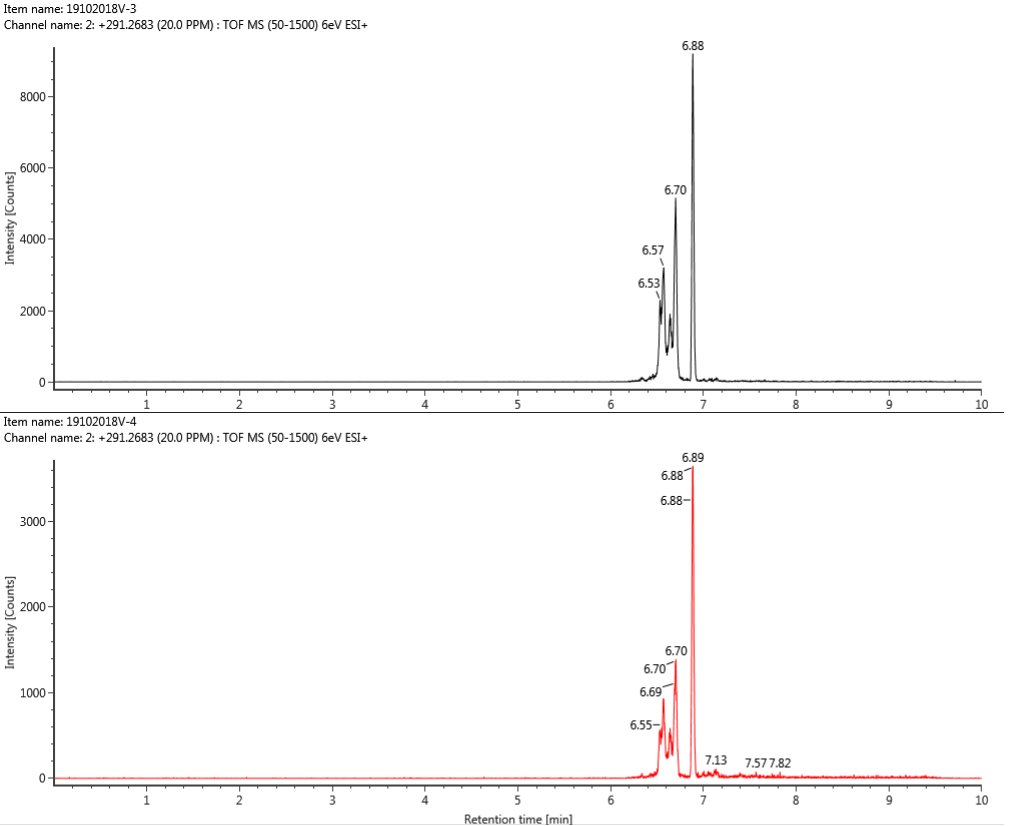
\includegraphics[scale=0.42]{images/291pos(p1,p2).png}
    \caption{Chromatograms of ion(m/z=291.2683) in bran powder and endosperm powder. Top (bran); bottom (endosperm).}
    \label{fig:291_barley}
\end{figure}

\begin{figure}[H]
    \centering
    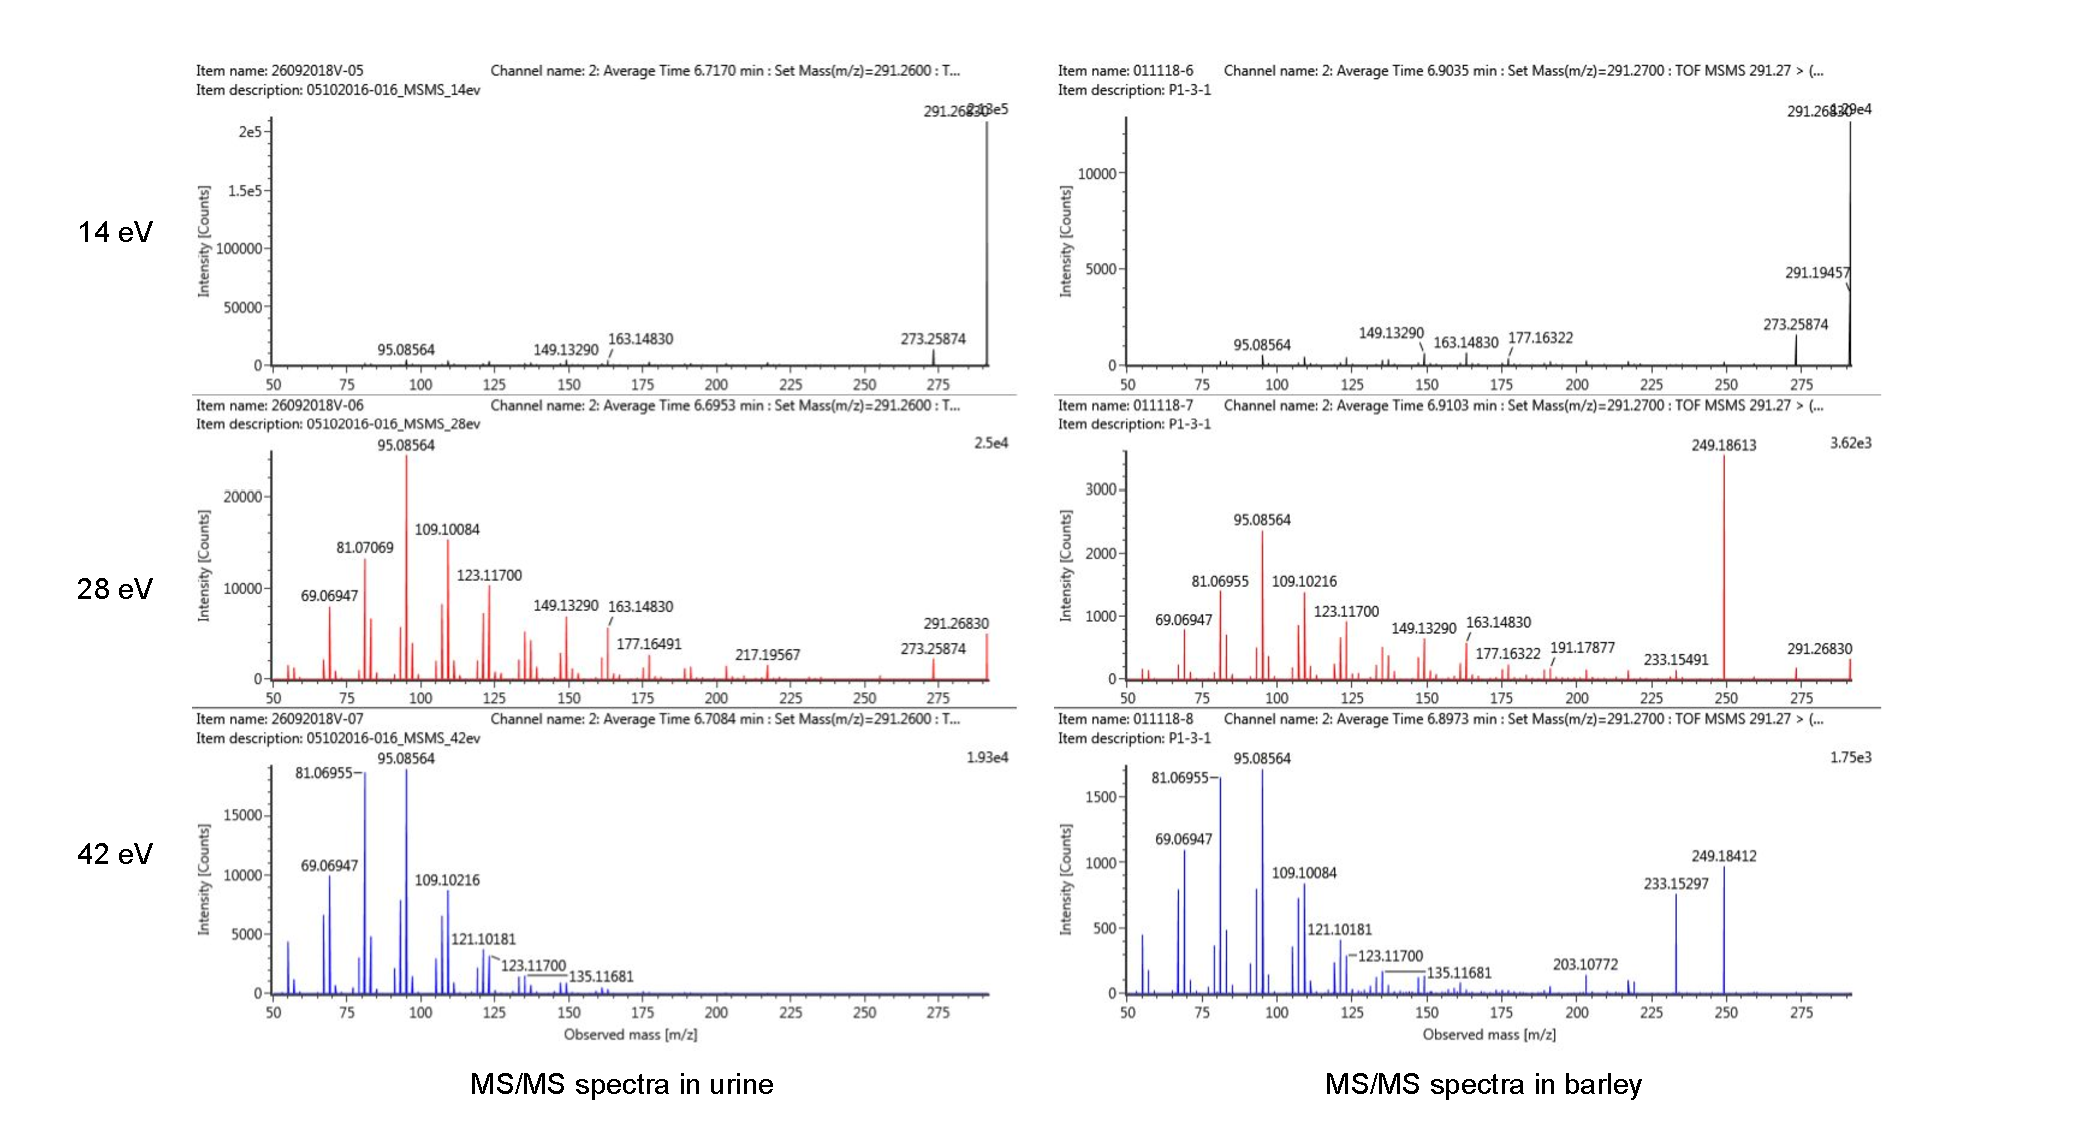
\includegraphics[scale=0.38]{images/ION291.pdf}
    \caption{MS/MS spectra of ion (m/z=291.2683) in urine and barley sample with different collision energies}
    \label{fig:MSMSION291}
\end{figure}
\begin{figure}[H]
    \centering
    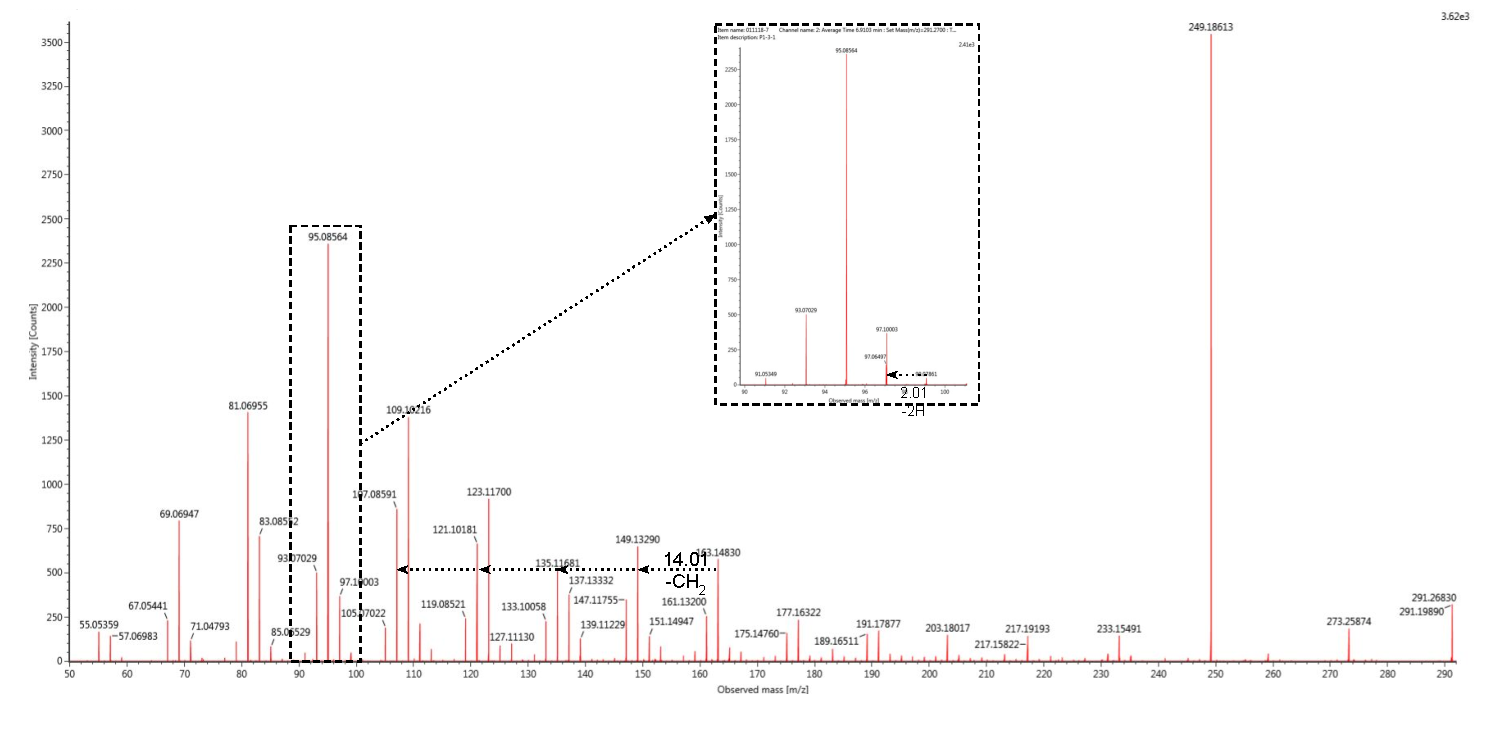
\includegraphics[scale=0.45]{images/Annotation-291.pdf}
    \caption{MS/MS spectra of ion(m/z=291.2683) in barley sample (Collision energy = 24 eV)}
    \label{fig:291_barley1}
\end{figure}



\begin{figure}[H]
    \centering
    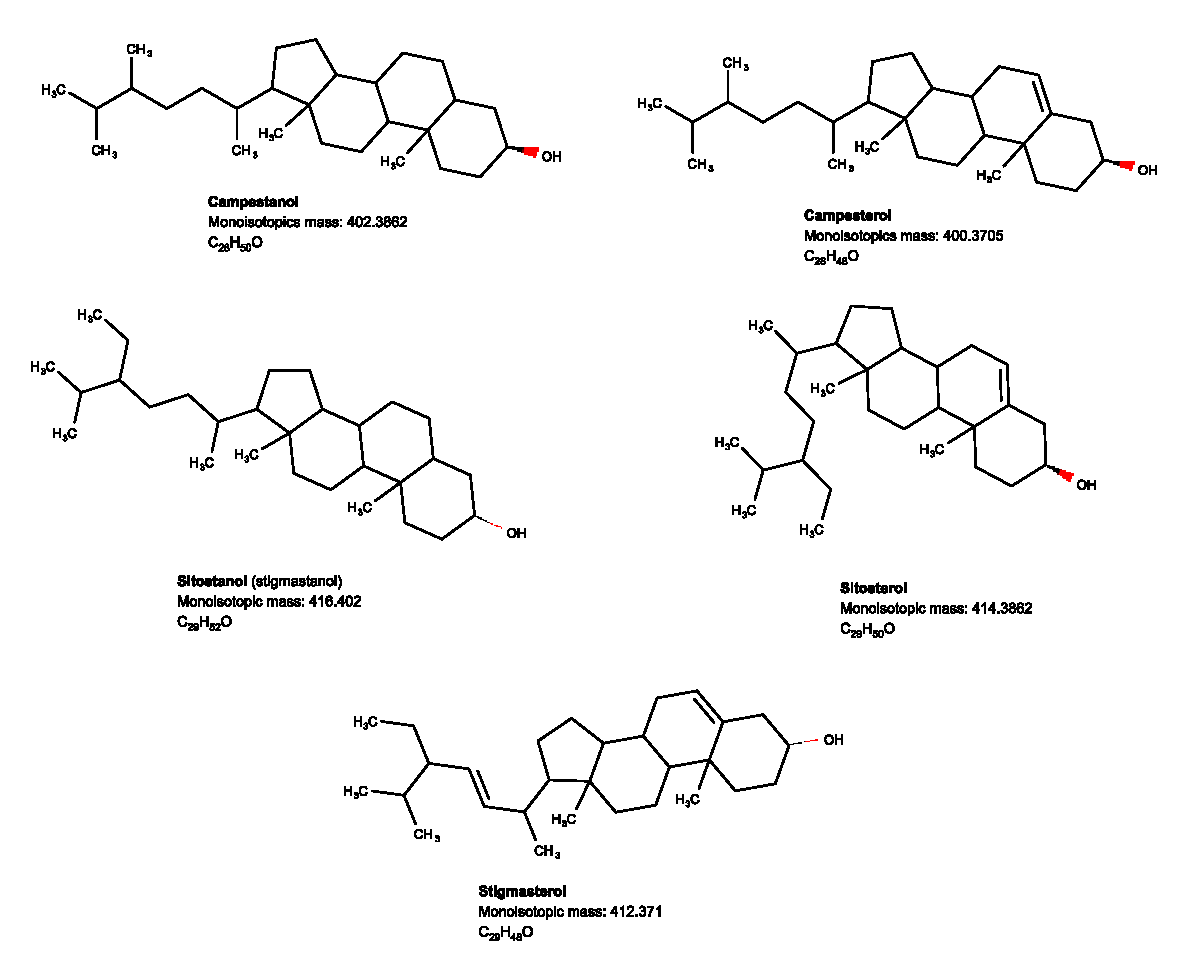
\includegraphics[scale=0.5]{images/5sterols_combined.eps}
    \caption{Major sterols in barley)}
    \label{fig:5sterol}
\end{figure}

Figure \ref{fig:5sterol} showed 5 major existed phytosterols in barley and were quantified\cite{sterol}. These 5 major types makes up around 90\% of total phytosterols\cite{sterol}. Still some minor sterols has not been identified yet.
We putatively identified the structure of this compound\ref{fig:putativesterol}. This proposal needs to be further validated.

\begin{figure}[H]
    \centering
    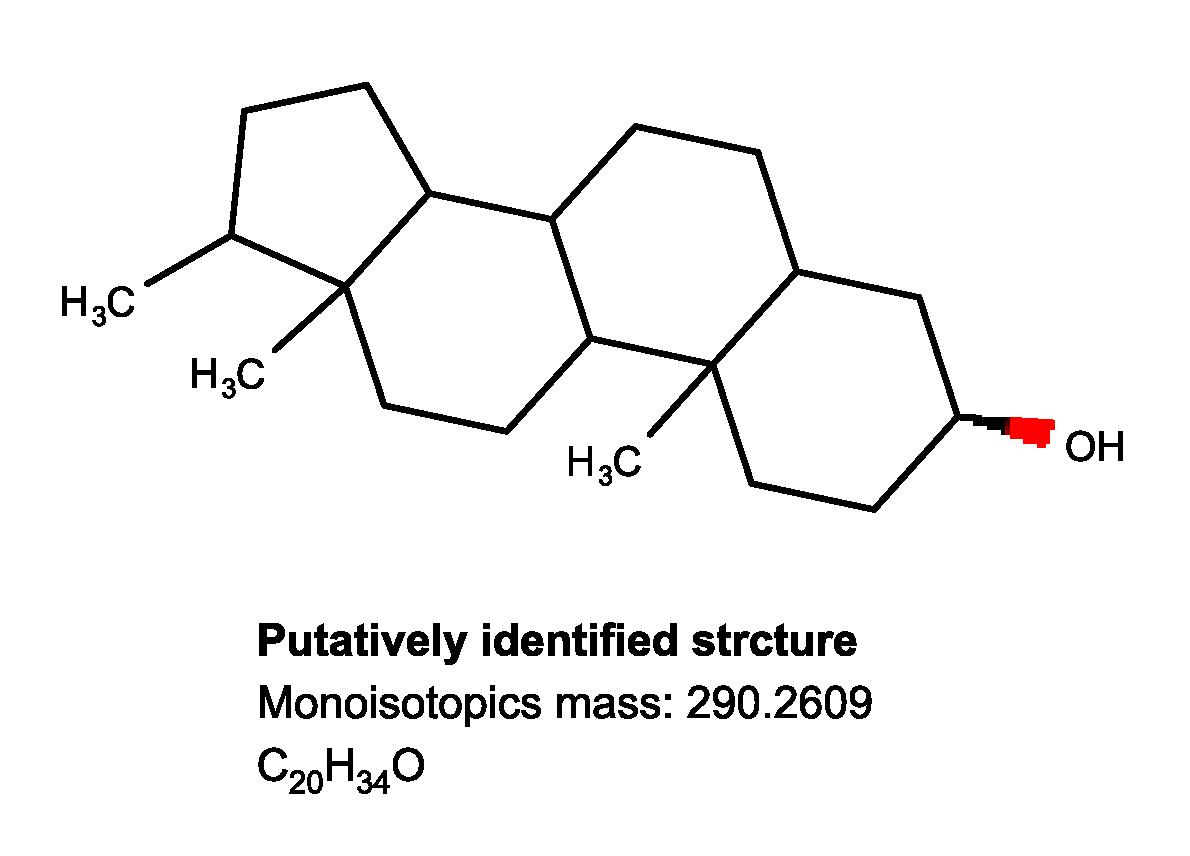
\includegraphics[scale=0.3]{images/possiblesterol.eps}
    \caption{Putatively identified structure}
    \label{fig:putativesterol}
\end{figure}

\section{Conclusions and Discussions}
An \acrshort{lc/ms} metabolomics study was perfomred to discover biomarkers for barley intake. 
\acrshort{lc/ms} was used to analyze whole grain barley (bran part and endosperm part separately). 
Further, \acrshort{lc/ms} was used to profile metabolome of urine from cross-over intervention. Multivariable data analysis (\acrshort{pca} and \acrshort{plsda}) was used to control data quality and select significant variables that can distinguish barley and wheat intake.

\begin{figure}[H]
    \centering
    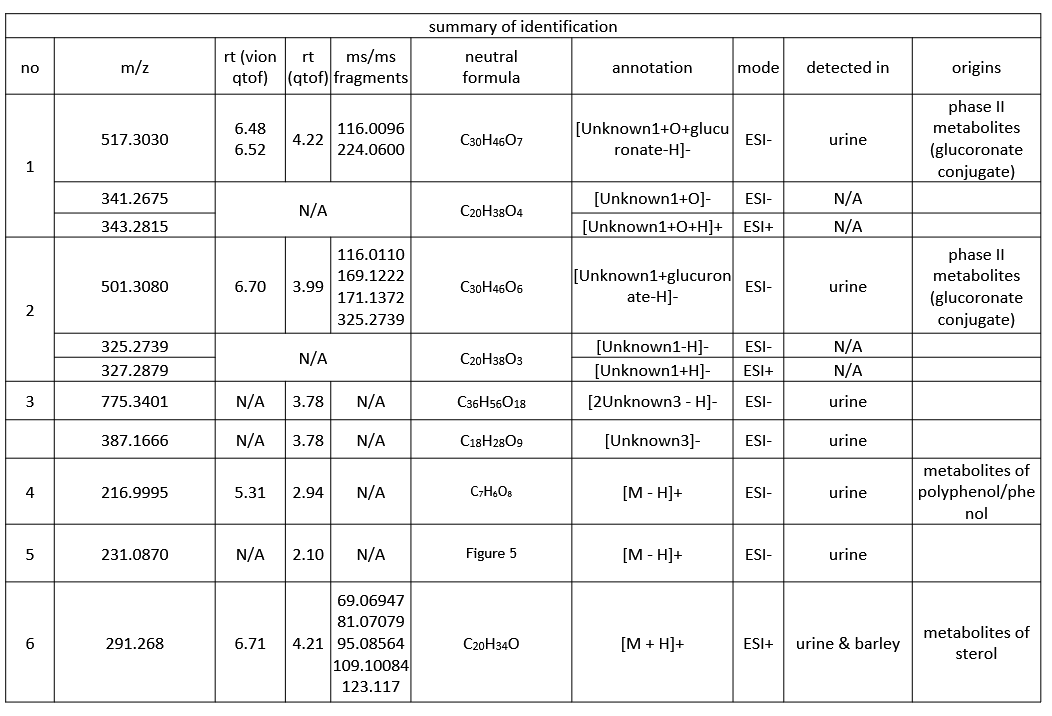
\includegraphics[scale=0.42]{images/idsummarybarley.PNG}
    \caption{Identification summary}
    \label{fig:idsummary}
\end{figure}


Further selected potential biomarkers were identified by \acrshort{ms/ms} and data-base searching. In the end, we proposed 6 potential biomarkers and putatively identified them for barley intake from urine shown in Figure \ref{fig:idsummary}. Within these 6 markers:
\begin{itemize}
    \item Two potential markers (m/z 231.0870, 775.3401), we can only report their molecular weight and possible molecular formulas.
    \item One marker was putatively identified as polyphenol or phenol metabolite.
    \item Two markers were putatively identified as glucoronate conjugates. Their unconjugated moleculars were not clear yet.
    \item One marker was putatively identified as sterol metabolite.
\end{itemize}

These markers should be further investigated and validated to confirm the structure.

These candidate biomarkers of barley intake appeared to be phytochemicals and their metabolites. 
Phytochemicals are chemical compounds produced by plants to help them thrive or thwart competitors, predators, or pathogens.
As a term, phytochemicals is generally used to describe plant compounds that are under research with unestablished effects on health and are not scientifically defined as essential nutrients.

In whole grain cereals, alkylresorcinols, benzoxazinoids, flavonoids, lignans and phytosterols were reported\cite{Koistinen2017}. From the perspective of systems biology, these phytochemicals are metabolites of plants controlled by gene expression. Therefore, different cereals, or more generally different plant-source food, should have their unique phytochemical profile. 

While human consumes the plant-source food, human's metabolome from biofluids  should also demonstrate unique pattern that can be tracked back to these phytochemicals. Therefore, unique metabolome pattern of phytochemical could differentiate and indicate plant-source food intakes. 

However, food is very complex biological and chemical mixtures. Phytochemicals only make up its small proportion. Identification, quantification methods and databases have not been established yet. Discovery of biomarkers for these plant-based phytochemicals could be progressed with more insights into these phytochemicals, but vice versa.
\section{Perspectives}
Plasma samples were also collected. They can be further studied to provide hints for compound identifications.
 
In this study, we detected some potential wheat intake biomarkers as well. 
These markers can also be identified and compared with barley markers. 
This could get some insights about specificity of cereal intake.
\section{Acknowledgements}
I sincerely acknowledge Gözde Gürdeniz's helpful, patient and detailed supervision for me. She was always available for my questions.

In addition, I acknowledge Lars' coordination job and sharing his knowledge of phytosterols and all fellows from Metabolomics group and all technicians. Without their kind help, I can not successfully finalize my project. I also thank the opponent (censor) Henrik to give his critical comments to the project.

I also thank Simon's Danish knowledge and his generous help in searching for the whole grain cereals. I acknowledge Inge sharing her knowledge and experience on whole grain cereals and Nikolin sharing her knowledge on Chemistry.

In the end, I acknowledge my girlfriend Jingyao, my grandfather Mr. Wang and all other dear family members who live in the time zone 6 or 7 hours ahead of me, but cares every details of my life.

This 15 ECTS project accounts only for 12.5\% of my master study. But it did open the door of a '\textit{brave new world}', Metabolomics, to me.

'O wonder!

How many goodly unknowns are there here!

How beauteous metabolome is! O brave new world,

That has barley in't!'


\clearpage
\section{Appendix}
\subsection{Chromatogram of Barley Flour}
\begin{figure}[h]
    \centering
    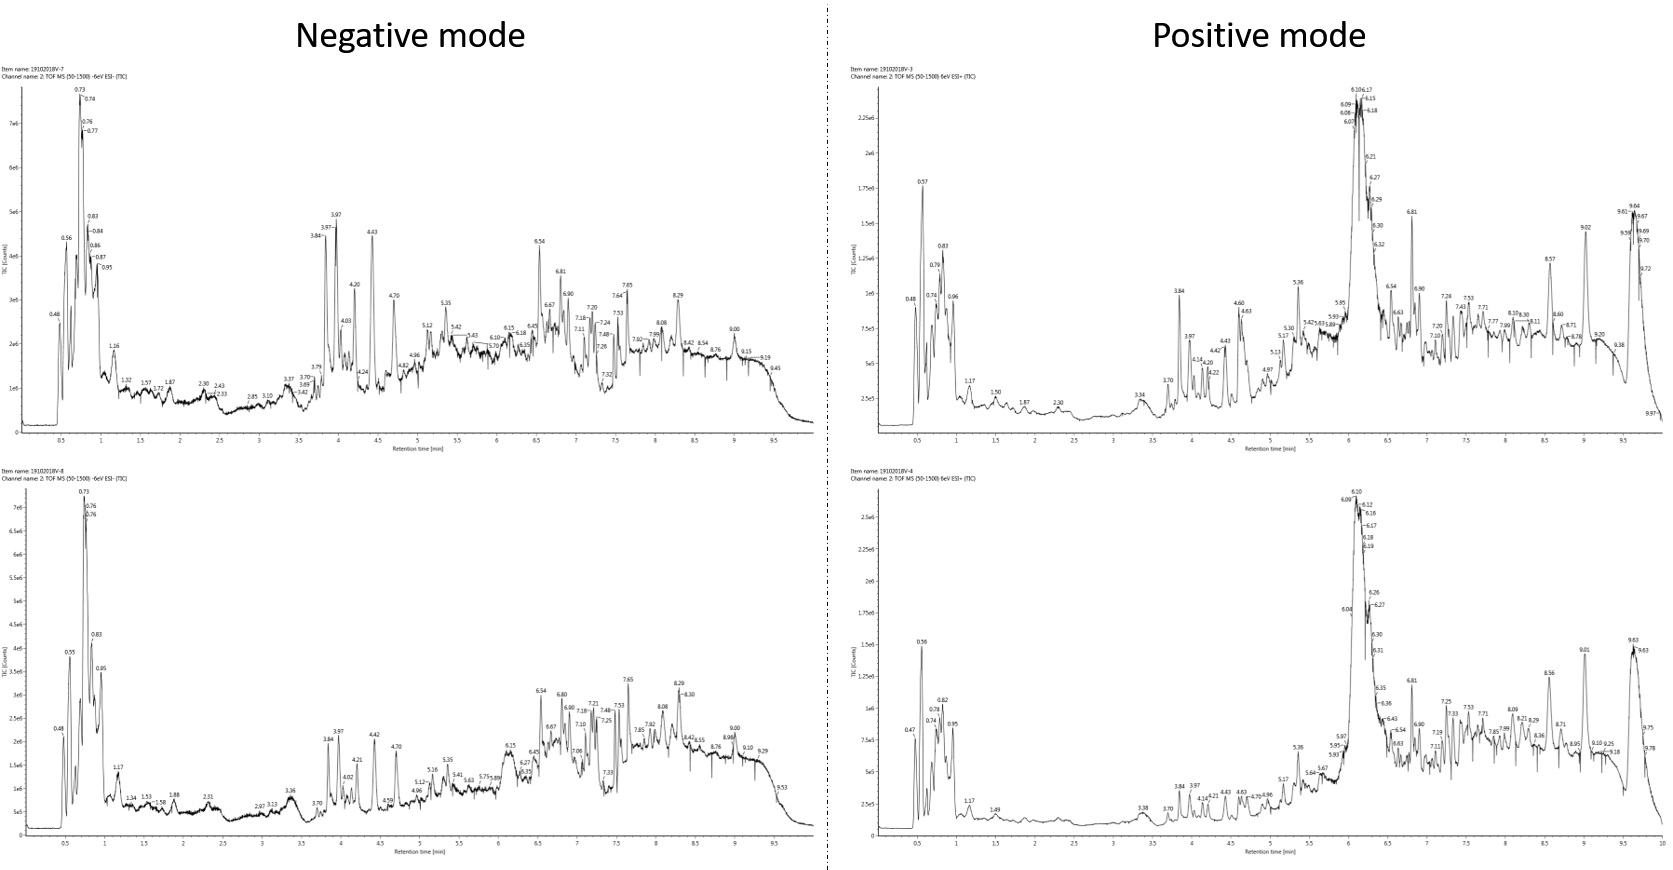
\includegraphics[scale=0.4]{images/chromatogram_barley_1.png}
    \caption{Chromatogram of Barley Flour (from top to the bottom: bran flour and endosperum flour)}
    \label{fig:chromatogram_barley}
\end{figure}

\clearpage
\subsection{\acrfull{ms/ms} spectra of phytosterols}
\acrshort{ms/ms} spectra of common phytosterols are shown in Figure \ref{fig:sterolmsms}, adapted from \cite{sterolms}
\begin{figure}[H]
    \centering
    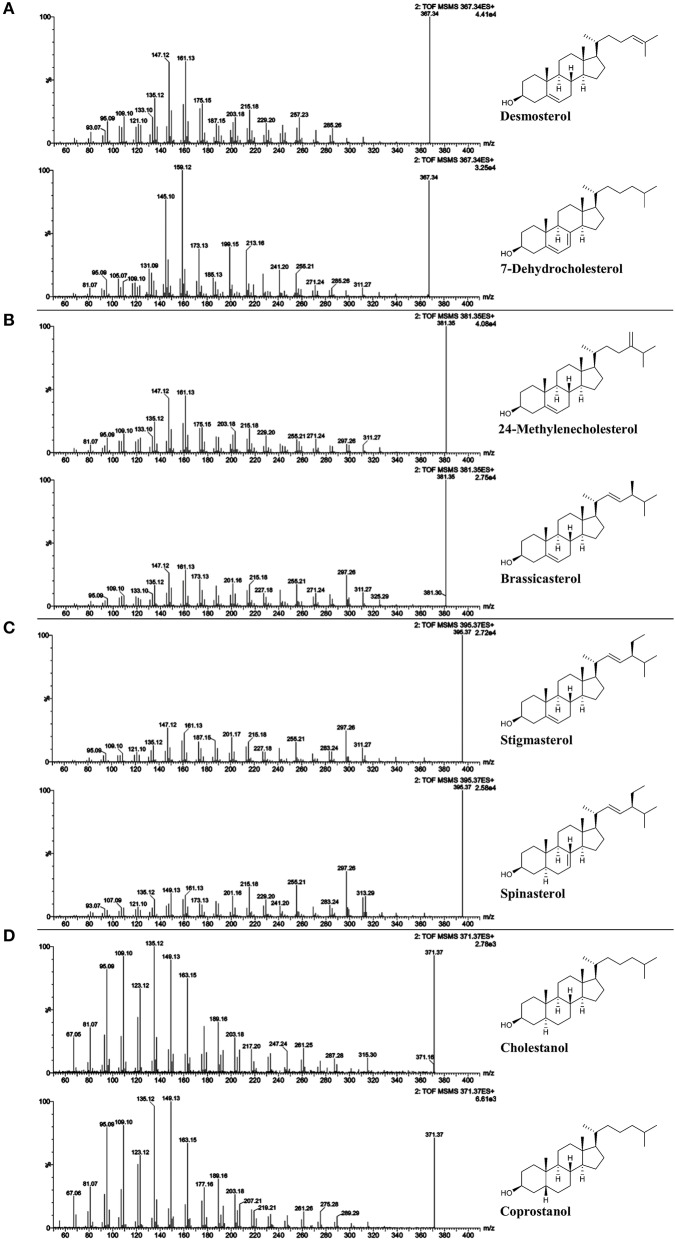
\includegraphics[scale=1]{images/sterolmsms.jpg}
    \caption{\acrshort{ms/ms} spectra of common phytosterols}
    \label{fig:sterolmsms}
\end{figure}
\clearpage
\printbibliography[
heading=bibintoc,
title={References}
]


\end{document}
